\documentclass[10pt,a4paper]{book}

\usepackage[utf8]{inputenc}
\usepackage[T1]{fontenc}
\usepackage[french]{babel}
%\renewcommand\sfdefault{phv}
\usepackage[left=2cm, right=2cm, bottom=1.85cm, top=1.5cm]{geometry}
\usepackage[skip=10pt plus1pt, indent=15pt]{parskip}
\usepackage{pgfplots}
\usepackage{fancyhdr}
\usepackage{framed}
\pagestyle{fancy}
\usepackage{hyperref}
\usepackage{multirow}
%\renewcommand{\headrulewidth}{1pt}
%\fancyhead[C]{\textbf{page \thepage}} 
\fancyhead[L]{Cours}
\fancyhead[R]{Terminale STMG}

\renewcommand{\footrulewidth}{1pt}
\fancyfoot[C]{\textbf{page \thepage}} 
\fancyfoot[L]{Lycée Jacques Brel}
\fancyfoot[R]{Année 2022-2023}

%%%%%%%%%%%%%%%%%%%%%%%%%%%%%%%%%%%%%%%%%%%%%%%%%%

%\newcommand{\TDoc}[1]{
%\begin{center}
%{\setlength{\fboxsep}{10pt}  % Ecart texte-boite
%\shadowbox{\textbf{\Large{#1}}}}
%\end{center}
%\vspace{1.5cm}}
    
 \usepackage{fancybox}   %pour l'encadré du titre shadowbox
 \usepackage{stmaryrd}   %pour utiliser correctement les crochets pour les ensembles de définitions
 \usepackage[normalem]{ulem}
 \usepackage{graphicx}
 %\usepackage{wrapfig} %texte coulé autour d'une image
 \usepackage{soul} % souligné
 \usepackage{nonfloat}
 \usepackage[standard]{ntheorem}
 \usepackage{array}
 \usepackage{arydshln}
 \usepackage{graphicx}
%MATHEMATIQUES
\usepackage{amsmath,amsfonts} 

\usepackage{tikz}
\newcommand{\N}{\mathbb{N}}
\newcommand{\Z}{\mathbb{Z}}
\newcommand{\D}{\mathbb{D}}
\newcommand{\Q}{\mathbb{Q}}
\newcommand{\R}{\mathbb{R}}
\newcommand{\Co}{\mathbb{C}}
\newcommand{\K}{\mathbb{K}}
\newcommand{\F}{\mathbb{F}}


%%%%%%%%%%%%%%%%%%%%%%%%%%%%%%%%%%%

\makeatletter
%%%%%%%%%%%%%%%%%%% debut fichier boiboites.sty %%%%%%%%%%%%%%%%%%%%%%
\RequirePackage{xkeyval}
\RequirePackage{tikz}
\usetikzlibrary{intersections}
\usetikzlibrary{positioning}
\usetikzlibrary{3d}
\RequirePackage{amssymb}

\define@key{boxedtheorem}{titlecolor}{\def\titlecolor{#1}}
\define@key{boxedtheorem}{titlebackground}{\def\titlebackground{#1}}
\define@key{boxedtheorem}{background}{\def\background{#1}}
\define@key{boxedtheorem}{titleboxcolor}{\def\titleboxcolor{#1}}
\define@key{boxedtheorem}{boxcolor}{\def\boxcolor{#1}}
\define@key{boxedtheorem}{thcounter}{\def\thcounter{#1}}
\define@key{boxedtheorem}{size}{\def\size{#1}}
\presetkeys{boxedtheorem}{titlecolor = black, titlebackground = white, background = white,%
                         titleboxcolor = black, boxcolor = black, thcounter=, size = .9\textwidth}{}

\newcommand{\couleurs}[1][]{%
    \setkeys{boxedtheorem}{#1}
    \tikzstyle{fancytitle} =[draw=\titleboxcolor, rounded corners, fill=\titlebackground,
                            text= \titlecolor]
    \tikzstyle{mybox} = [draw=\boxcolor, fill=\background, very thick,
                        rectangle, rounded corners, inner sep=10pt, inner ysep=20pt]
}


%Commande generique pour faire un joli encadre
\newsavebox{\boiboite}
\newcommand{\titre}{Titre}
\newenvironment{boite}[2][]%
    {%
    \renewcommand{\titre}{#2}
    \couleurs[#1]
    \begin{lrbox}{\boiboite}%
     \begin{minipage}[!h]{\size}
    }%
    {%
     \end{minipage}
    \end{lrbox}
    \begin{center}
    \begin{tikzpicture}
    \node [mybox] (box){\usebox{\boiboite}};
    \node[fancytitle, right=10pt] at (box.north west) {\titre};
    \end{tikzpicture}
    \end{center}
    }

\newcommand{\newboxedtheorem}[4][]{%
    \couleurs[#1]
    \@ifnotempty{#4}{%
      \@ifundefined{the#4}{\@ifundefined{\thcounter}{\newcounter{#4}}{%
      \newcounter{#4}[\thcounter ] } } { }%
    }
    \newenvironment{#2}[1][]{%
    \@ifnotempty{#4}{\refstepcounter{#4}}
    \begin{boite}[#1]{\textbf{#3\@ifnotempty{#4}{ \csname the#4\endcsname}}\@ifnotempty{##1}{
    (##1)}}
    }%
    {%
    \end{boite}
    }
}

\newcommand{\newboxedtheoreme}[4][]{%
    \couleurs[#1]
    \@ifnotempty{#4}{%
      \@ifundefined{the#4}{\@ifundefined{}{}{%
      } } { }%
    }
    \newenvironment{#2}[1][]{%
    \@ifnotempty{#4}{\refstepcounter{#4}}
    \begin{boite}[#1]{\textbf{#3\@ifnotempty{#4}{ \csname the#4\endcsname}}\@ifnotempty{##1}{
    (##1)}}
    }%
    {%
    \end{boite}
    }
}
%%%%%%%%%%%%%%%%%%%% end fichier boiboites.sty %%%%%%%%%%%%%%%%%%%%%%
\makeatother
\newboxedtheorem{theo}{Théorème}{theorem}
\newboxedtheorem{de}{D\'efinition}{theorem}
\newboxedtheorem{prop}{Propriété}{theorem}
\newboxedtheorem{pro}{Proposition}{theorem}
\newboxedtheorem{ton}{Notation}{theorem}
\newtheorem{exo}{Exercice}
\newboxedtheorem{exe}{Exemple}{theorem}
\newboxedtheorem{cor}{Corolaire}{theorem}
\newboxedtheoreme{conc}{Conclusion}{theorem*}
\newboxedtheoreme{demo}{\textbf{Démonstration guidée}}{theorem}
%%%%%%%%%%%%%%%%%%%%%%%%%%%%%%
%%%%%%%%%%%%%%%%%%%%%%%%%%%%%
\newlength{\longA}
\newlength{\longB}
\newenvironment{BoiteShadow}[3][\linewidth]{%
\addtolength{\longA}{#2}
\addtolength{\longB}{#3}
\begin{Sbox}\begin{minipage}{#1}}%
{\end{minipage}\end{Sbox}%
\setlength{\fboxsep}{\longA}
\setlength{\shadowsize}{\longB}
\shadowbox{\unhbox\@Sbox}\par}
\makeatother
\author{Augustin WENGER}

\title{Cours de Terminale STMG 2 2022-2023}
\date{\today}

%%%% fin du préambule, on passe au contenu : tout le texte entre
%%%% \begin{document} et \end{document} 

\begin{document}
\maketitle
\tableofcontents
\chapter{Suites arithmétiques et géométriques}

\section{Suites : les bases}


\subsection{Vocabulaire}

\begin{de}[Rappel]
    Une \underline{suite numérique} est une liste \textbf{infinie} et \textbf{numérotée} (c'est à dire classée selon un certain ordre) d'éléments.
 Ces éléments sont appelés les \underline{termes} de la suite.
\end{de}


Notation : Si l'on appelle la suite $u$, on note pour tout entier naturel $n$   $u_n$ le $n$-ième terme de la suite.


\textit{Par exemple, si $u$ est la suite des nombres pairs strictement positifs, le $4$-ième terme de la suite est appelé $u_4$ et vaut $8$. On montre les valeurs des termes de cette suite dans le tableau ci dessous }

{
\centering
    \begin{tabular}{|c|c|c|c|c|c|c|c|c|}
        \hline
         $u_1$ & $u_2$ & $u_3$ & $u_4$ & $u_5$ & \ldots & $u_n$ & \ldots\\
        \hline
         $2$ & $4$ & $6$ & $8$ & $10$ & \ldots & $2n$ & \ldots \\ 
        \hline
    \end{tabular}\par
}

Remarque : Une suite est entièrement définie par l'ensemble de ses termes. Si deux suites ont \textbf{tous} leur termes égaux, elles sont égales.

\subsection{Décrire une suite}

Pour exprimer la formule d'une suite, il faut donner une méthode pour calculer chacun de ses termes. Pour cela, deux manières sont possibles :
    \begin{enumerate}
      \item Méthode du \underline{terme général} : On donne directement la formule pour calculer chaque terme. 

      \item Méthode \underline{récursive} : On initialise la suite en donnant le premier terme de la suite, puis on donne une formule pour calculer chacun des termes qui suit en fonction des nombres qui précèdent.
    \end{enumerate}
    
    On peut par exemple dire de la suite $u$ des entiers pairs décrite ci-dessus:
    
      {
      \centering
      Méthode du terme général : \textit{Le terme général de la suite $u$ (définie plus haut) est $u_n=2n$}
      \par

ou
    
      Méthode récursive : \textit{La suite $u$ est définie par $u_1=1$ et pour $n\geq1$, $u_{n+1}=u_n+1$}\par
      }

\subsection{Sens de variation : Suite croissante ou décroissante}

\begin{de}[Rappel]
Une suite est dite \underline{croissante} si ses termes sont de plus en plus grands, c'est à dire si $u_{n+1}$ est \textbf{toujours} supérieur ou égal à $u_n$ quel que soit le choix de l'entier $n$.

On écrit : pour tout $n \geq 1$, $u_{n+1} \geq u_n$
\end{de}

Remarques :
\begin{itemize}
    \item Si on a l'inégalité stricte : pour tout $n \geq 1$, $u_{n+1} > u_n$, on dit que la suite est \underline{strictement} croissante
    \item Si les termes sont de plus en plus petits, c'est à dire si pour tout $n \geq 1$, $u_{n+1} \leq u_n$  on dit que la suite est décroissante.
    \item Pour vérifier si une fonction est (dé)croissante, on regarde si $u_{n+1}$ est plus grand ou plus petit que $u_n$, par exemple en calculant le signe de $u_{n+1} - u_n$. Si le signe est toujours le même, la suite est croissante (si le signe est toujours positif) ou décroissante (si le signe est toujours négatif).
\end{itemize}


Exemple : La suite des entiers pairs $u_n=2n$ est strictement croissante. En effet, pour tout $n \geq 1$, $u_{n+1} - u_n = 2(n+1) - 2n= 2 (n+1-n) = 2 > 0$. $u_{n+1}$ est donc toujours strictement plus grand que $u_n$, ce qui est la définition de la croissance stricte.



\section{Suites arithmétiques}

Intuitivement, les suites arithmétiques sont les suites où pour passer d'un terme à l'autre, on augmente (ou diminue) toujours de la même quantité.

\newcommand{\insertph}[1]{%
 \tikz[remember picture] \node[inner sep=0pt,minimum height=10pt](#1){};} 
 

{
\centering
    \begin{tabular}{|c|c|c|c|c|c|c|c|c|}
        \hline
         $u_1$ & $u_2$ & $u_3$ & $u_4$ & \ldots & $u_n$ & $u_{n+1}$ & \ldots\\
        \hline
         $2\insertph{n1}$ & $\insertph{n2}4\insertph{n3}$ & $\insertph{n4}6\insertph{n5}$ & $\insertph{n6}8$ &  \ldots &  $u_n$\insertph{n7} & $\insertph{n8}u_{n+1}$  & \ldots \\ 
        \hline
    \end{tabular}\par
}

\tikz[remember picture,overlay]\draw[->,blue] ([yshift=-2mm] n1.south) to  [out=-45,in=-150] node[below]{+2} ([yshift=-2mm] n2.south) ; 
\tikz[remember picture,overlay]\draw[->,blue] ([yshift=-2mm]n3.south) to[out=-45,in=-150] node[below]{+2}  ([yshift=-2mm]n4.south); 
\tikz[remember picture,overlay]\draw[->,blue] ([yshift=-2mm]n5.south) to[out=-45,in=-150] node[below]{+2} ([yshift=-2mm]n6.south); 
\tikz[remember picture,overlay]\draw[->,blue] ([yshift=-2mm]n7.south) to[out=-45,in=-150] node[below]{+2} ([yshift=-2mm]n8.south); 


On va voir que cette catégorie de suites a deux caractéristiques importantes :
\begin{itemize}
    \item Elles se retrouvent souvent dans les problèmes concrets :
    \begin{itemize}
        \item On économise de l'argent en plaçant une somme fixe chaque semaine
        \item Un objet s'éloigne d'un autre à une vitesse fixe
    \end{itemize}
    \item On peut facilement obtenir des formules pour calculer un terme donné de la suite, ou même la somme de termes consécutifs de la suite.
\end{itemize}

\subsection{Définition}

\begin{de}
Une \underline{suite arithmétique} est une suite où chaque terme est obtenu en rajoutant le même nombre réel qu'on appelle \underline{raison}) au terme précédent.
Formellement, une suite $u$ est dite géométrique de raison $q$ si pour tout entier $n$ tel que $u_n$ est défini, on a la relation : $u_{n+1} = u_n + r$ 
\end{de}

On déduit de cette définition une première technique pour montrer qu'une suite est arithmétique : On calcule la différence de deux termes consécutifs quelconques : $u_{n+1} - u_n$. Si on trouve quelque chose qui ne dépend \textbf{pas} de $n$, la suite est arithmétique.


\subsection{Propriétés de base}

\begin{prop}

Dans la représentation graphique d'une suite arithmétique, tous les points représentants la suite sont alignés
\end{prop}

\begin{figure}[!h]
  \caption{Exemple : représentation graphique de la suite $u_n=2n$}
    \centering
    \begin{tikzpicture}
      \begin{axis}[ 
        xlabel={n (Numéro du terme)},
        ylabel={$u_n$ (Valeur du terme)},
        xmin=1, xmax=10,
        ymin=0, %ymax=55,
        xtick={1,...,10},
        domain={1:10},
        samples=10
      ]
        \addplot[only marks, mark=x, blue] {2*x}; 
       % \addplot[only marks, red] {21-x}; 
      \end{axis}
    \end{tikzpicture}
\end{figure}

\subsubsection{Calcul du terme général d'une suite arithmétique}

Quand on connaît la raison d'une suite, il suffit de connaître un seul terme et l'on peut calculer tous les termes de la suite :

\begin{prop}

Si on connaît le premier terme $u_1$ d'une suite arithmétique et sa raison $r$, la formule de son terme général est donnée par $u_n=u_1+r(n-1)$.
\end{prop}

Explication : A chaque passage d'un terme à un suivant, on ajoute $r$. Entre $u_1$ et $u_n$, il y a $n-1$ passages. Donc, comme on rajoute $r$ à chaque étape, on obtient un accroissement de $r(n-1)$ au total.

Exemple : $u_1=2$ et $r=2$ (toujours le même exemple). On veut calculer le $5$-ème terme de la suite :

{
\centering
    \begin{tabular}{|c|c|c|c|c|c|}
        \hline
        $u_1$ & $u_2$ & $u_3$ & $u_4$  & $u_5$ & \ldots \\
        \hline
         $2\insertph{n1}$ & $\insertph{n2}4\insertph{n3}$ & $\insertph{n4}6\insertph{n5}$ & $\insertph{n6}8\insertph{n7}$ &  \ $\insertph{n8}10$  & \ldots \\ 
        \hline
    \end{tabular}\par
}

\tikz[remember picture,overlay]\draw[->,blue] ([yshift=-2mm] n1.south) to  [out=-45,in=-150] node[below]{+2} ([yshift=-2mm] n2.south) ; 
\tikz[remember picture,overlay]\draw[->,blue] ([yshift=-2mm]n3.south) to[out=-45,in=-150] node[below]{+2}  ([yshift=-2mm]n4.south); 
\tikz[remember picture,overlay]\draw[->,blue] ([yshift=-2mm]n5.south) to[out=-45,in=-150] node[below]{+2} ([yshift=-2mm]n6.south); 
\tikz[remember picture,overlay]\draw[->,blue] ([yshift=-2mm]n7.south) to[out=-45,in=-150] node[below]{+2} ([yshift=-2mm]n8.south); 
\tikz[remember picture,overlay]\draw[->,red,label = {Lutsa}] ([yshift=-2mm]n1.south) to[out=-100,in=-100] node[below]{$4$ augmentations de $2$ = Augmentation totale de $8$} ([yshift=-2mm]n8.south); 

\vspace{20 mm}

Attention : Si le premier terme n'est pas numéroté $u_1$ mais $u_0$ (ou autre), il faut ajuster le nombre d'étapes pour passer du premier terme à celui qu'on veut calculer.  Par exemple, il y a 5 étapes entre $u_0$ et $u_5$. Plus généralement, entre un terme $u_n$ et un terme $u_N$, avec $n \leq N$ entiers, il y a $N-n$ étapes.

Donc, savoir d'une suite qu'elle est arithmétique \textbf{et} connaître au moins un terme \textbf{et} connaître sa raison suffisent à pouvoir calculer tous les termes de la suite. On dit que ces informations sont \underline{caractéristiques} de la suite (les connaître suffit à connaître la suite dans sa globalité).

C'est même encore plus fort que ça : on peut calculer la raison à partir de la donnée de deux termes de la suite.

\begin{prop}
    Si l'on connaît deux termes distincts $u_n$ et $u_m$ d'une suite arithmétique $u$ (avec $n \neq m$), on peut calculer sa raison $r$ et la formule nous est donnée par : $r = \frac{u_m-u_n}{m-n}$
\end{prop}

Par conséquent, il suffit de connaître 2 informations sur une suite arithmétique pour connaître cette suite :
\begin{itemize}
    \item Sa raison et un terme quelconque
    \item Deux termes quelconques de la suite.
\end{itemize}

\subsubsection{Sens de variation}

Le sens de variation d'une suite arithmétique est intuitivement simple à déterminer : si on augmente entre un terme et le terme suivant (c'est à dire si la raison de la suite est positive), la suite est croissante. Si au contraire on diminue entre un terme et le suivant, la suite est décroissante. Plus précisément :

\begin{prop}
    Si la raison $r$ d'une suite arithmétique est strictement positive, cette suite arithmétique est strictement croissante.
    Si la raison $r$ d'une suite arithmétique est strictement négative, cette suite arithmétique est strictement décroissante.
\end{prop}


On fait le lien avec les fonctions affines : 
\begin{itemize}
    \item Des représentations en points alignés. Mais si on tire un trait ! 
    \item la formule du terme général : $u_n=an+b$ rappelle $f(x)=ax+b$ les fonctions affines ou $y=ax+b$ les équations de droite (non-verticales) du plan
    \item Au même titre que connaître deux points d'une droite permet de caractériser une droite (il existe une et une seule droite passant par deux points), il suffit de connaître deux termes d'une suite pour connaître la suite
    \item La raison, ça fait penser au taux d'accroissement d'une fonction affine (qui est la pente ou le coefficient directeur de la droite), c'est d'ailleurs la même formule, et si l'on connaît sa valeur, il suffit alors d'un terme de la suite (équivalent d'un point d'une droite).
\end{itemize}

\subsection{Moyenne arithmétique}

La moyenne arithmétique de deux nombres réels est ce qu'on appelle couramment la moyenne (mais comme on verra une autre sorte de moyenne, la moyenne géométrique, on précisera désormais de quelle moyenne on parle

\begin{de}
    La \underline{moyenne arithmétique} de deux nombre est la moitié de leur somme, c'est à dire, si l'on note les deux nombres $a$ et $b$, le nombre $\frac{a+b}{2}$
\end{de}

\subsubsection{Lien avec les suites arithmétiques}

On se demande ici si trois nombres $a$,$b$ et $c$ peuvent être trois termes consécutifs d'une suite arithmétique. Pour cela, il faut que l'accroissement entre deux termes soit constant.

{
\centering
    \begin{tabular}{|c|c|c|c|}
        \hline
        $u_1$ & $u_2$ & $u_3$ & \ldots \\
        \hline
         $\hspace{10pt}a\insertph{n1}\hspace{10pt} $ & $\hspace{10pt} \insertph{n2}b\insertph{n3}\hspace{10pt} $ & $\hspace{10pt} \insertph{n4}c \hspace{10pt} $ & \ldots \\ 
        \hline
    \end{tabular}\par
}

\tikz[remember picture,overlay]\draw[->,blue] ([yshift=-2mm] n1.south) to  [out=-45,in=-150] node[below]{$+b-a$} ([yshift=-2mm] n2.south) ; 
\tikz[remember picture,overlay]\draw[->,blue] ([yshift=-2mm]n3.south) to[out=-45,in=-150] node[below]{$+c-b$}  ([yshift=-2mm]n4.south);

Les termes $a$,$b$ et $c$ peuvent être trois termes consécutifs d'une suite arithmétique si et seulement si l'accroissement est constant, c'est à dire si $b-a=c-b$. On peut formuler cela à l'aide de la définition d'une moyenne arithmétique : $b$ doit être "au milieu" de $a$ et de $c$ dans le sens suivant :

\begin{prop}
    Trois nombres $a$,$b$ et $c$ sont trois termes consécutifs (dans cet ordre) d'une suite arithmétique si et seulement si $b$ est la moyenne arithmétique de $a$ et de $c$.
\end{prop}



\subsection{Somme de termes consécutifs d'une suite arithmétique}

En plus de la formule du terme général d'une suite arithmétique, il existe une formule pour calculer la somme des termes consécutifs d'une suite arithmétique :

\begin{prop}
    La somme des termes consécutifs d'une suite arithmétique est égale au nombre de termes dont on fait la somme multipliée par la moyenne arithmétique du premier et du dernier terme.
    Formellement, si $n$ et $p$ sont des entiers avec $n \leq p$, et que $u$ est une suite arithmétique, on a:
    \[  \sum_{i=n}^{p} u_i= u_n + u_{n+1} + \ldots  + u_{p-1} + u_p = \frac{(u_n+u_p)}{2} \times (p-n+1)
    \]
\end{prop}

Explication : N'importe quelle somme de nombres est toujours égale à la moyenne de ses termes multipliée par le nombre de termes (par définition de la moyenne). Or, dans le cas d'une suite arithmétique, les termes augmentent (ou diminuent) toujours de la même quantité, par conséquent si l'on "groupe" les termes en associant le premier au dernier, le deuxième à l'avant-dernier, on obtient toujours la même somme. On peut le voir en utilisant les formules données plus haut si l'on suppose que la raison est $r$:


\begin{tabular}{ccccc}
$u_n + u_p $&$=$ &$  u_n  +  u_n + (p-n) \times r $&$=$ & $ 2u_n + (p-n)r$ \\
$u_{n+1} + u_{p-1} $&$=$&$u_n + r  +  u_n + (p-1-n) \times r $&$=$&$2u_n + (p-n)r$
     & 
\end{tabular}

Et ainsi de suite pour tous les termes. On peut donc "retourner" la suite et l'ajouter à elle même, et l'on obtient alors une suite de termes constants, comme l'illustre la figure  \ref{fig:sumarith}

\begin{figure}[htbp]
\centering
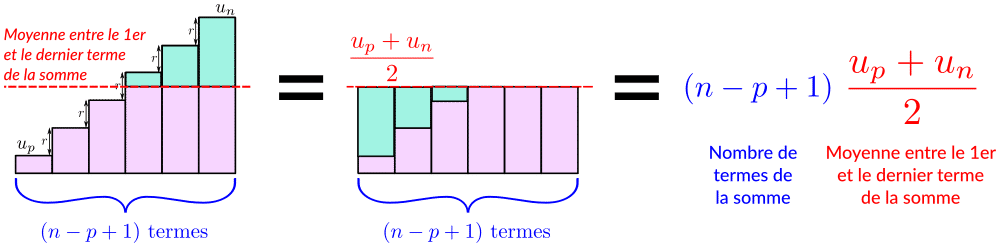
\includegraphics[width=1.0\textwidth]{suites-arithmetiques-somme.png}
\caption{Illustration du principe de la somme de termes d'une suite arithmétique de raison r}
\label{fig:sumarith}
\end{figure}


A retenir :

\begin{itemize}
    \item Mots à savoir définir : suite arithmétique, raison d'une suite arithmétique, moyenne arithmétique
    \item La définition d'une suite arithmétique : permet de vérifier si une suite est arithmétique ou non
    \item La formule du terme général : $u_n = u_1 + (n-1) \times r$
    \item Trouver la raison d'une suite arithmétique à partir de deux termes distincts donnés
    \item Formule de la somme de termes consécutifs d'une suite arithmétique.
\end{itemize}



\section{Suites géométriques}

Pour passer d'un terme au suivant dans une suite géométrique, on ajoutait toujours la même quantité, qui était la raison de la suite. Pour passer d'un terme au terme suivant dans une suite géométrique, on va toujours \textbf{multiplier} par la même quantité : dans l'exemple ci-dessous, on multiplie un terme par 2 pour passer au suivant.


{
\centering
    \begin{tabular}{|c|c|c|c|c|c|c|c|c|}
        \hline
         $u_1$ & $u_2$ & $u_3$ & $u_4$ & \ldots & $u_n$ & $u_{n+1}$ & \ldots\\
        \hline
         $2\insertph{n1}$ & $\insertph{n2}4\insertph{n3}$ & $\insertph{n4}8\insertph{n5}$ & $\insertph{n6}16$ &  \ldots &  $u_n$\insertph{n7} & $\insertph{n8}u_{n+1}$  & \ldots \\ 
        \hline
    \end{tabular}\par
}

\tikz[remember picture,overlay]\draw[->,blue] ([yshift=-2mm] n1.south) to  [out=-45,in=-150] node[below]{$\times 2$} ([yshift=-2mm] n2.south) ; 
\tikz[remember picture,overlay]\draw[->,blue] ([yshift=-2mm]n3.south) to[out=-45,in=-150] node[below]{$\times 2$}  ([yshift=-2mm]n4.south); 
\tikz[remember picture,overlay]\draw[->,blue] ([yshift=-2mm]n5.south) to[out=-45,in=-150] node[below]{$\times 2$} ([yshift=-2mm]n6.south); 
\tikz[remember picture,overlay]\draw[->,blue] ([yshift=-2mm]n7.south) to[out=-45,in=-150] node[below]{$\times 2$} ([yshift=-2mm]n8.south);

On va voir qu'on va pouvoir obtenir comme dans le cas des suites arithmétiques des formules pour calculer le terme général d'une telle suite, son sens de variation, et la somme de termes consécutifs. Certaines formules ressembleront à celles des suites arithmétiques, d'autres moins.

Mais d'abord, petit rappel sur les différentes manières de parler d'une évolution multiplicative.

\subsection{Différentes manière d'exprimer une progression multiplicative}

Il existe plusieurs manières d'exprimer qu'une quantité est multipliée par un certain nombre.

Par exemple, si le prix d'un manteau passe de 100€ à 80€ dans une période de soldes, on peut dire que le prix baisse de 20€ (c'est la vision en \textbf{variation absolue}. On peut dire l'une des  choses suivantes si l'on adopte une vision multiplicative :

\begin{itemize}
    \item Le prix du manteau diminue de 20\%, on dit que $-20\%$ est son \textbf{taux d'évolution}
    \item Le prix du manteau est multiplié par un \textbf{coefficient multiplicateur} de $0{,}8$
\end{itemize}

\begin{de}
    Soit une quantité observée, qui passe d'une valeur initiale VI à une valeur finale VF.
    \begin{itemize}
        \item La \underline{variation absolue} est donnée par $VF - VI$ (vision additive)
        \item Le \underline{taux d'évolution} est donné par $\frac{VF-VI}{VI}$ (On l'exprime souvent en pourcentage)
        \item Le \underline{coefficient multiplicateur} est donné par 
        $\frac{VF}{VI}$. C'est le nombre par lequel on multiplie VI pour obtenir VF.
    \end{itemize}
\end{de}

\begin{prop}
    Pour passer du coefficient multiplicateur au taux d'évolution, on retire $1$ au coefficient multiplicateur. \newline
    Pour passer du taux d'évolution au coefficient multiplicateur, on rajoute $1$ au taux d'évolution.
\end{prop}

\subsubsection{Evolutions successives}

Si deux évolutions successives ont lieu, \textbf{l'évolution totale a pour coefficient multiplicateur le produit des coefficients multiplicateurs.}

Par exemple, une hausse du prix du gaz de 10\% (Coefficient multiplicateur de $1{,}1$) suivie d'une hausse de 50\% ((Coefficient multiplicateur de $1{,}5$) correspond à un coefficient multiplicateur total de $1{,}1 \times 1{,}5 = 1{,}65$ soit une hausse de 65\%


{
\centering
    \begin{tabular}{|c|c|c|c|}
        \hline
        Année& 1 & 2 & 3 \\
        \hline
         Prix du gaz (base 100 en année 1)& $\insertph{n0}100\insertph{n1}$ & $\insertph{n2}110\insertph{n3}$ & $\insertph{n4}165\insertph{n5}$  \\ 
        \hline
    \end{tabular}\par
}

\tikz[remember picture,overlay]\draw[->,blue] ([yshift=-2mm] n1.south) to  [out=-45,in=-150] node[below]{$\times 1{,}1$} ([yshift=-2mm] n2.south) ; 
\tikz[remember picture,overlay]\draw[->,blue] ([yshift=-2mm]n3.south) to[out=-45,in=-150] node[below]{$\times 1{,}5$}  ([yshift=-2mm]n4.south); 
\tikz[remember picture,overlay]\draw[->,red,label = {Lutsa}] ([yshift=-2mm]n0.south) to[out=-100,in=-100] node[below]{$\times 1{,}65$} ([yshift=-2mm]n5.south); 

\vspace{1cm}
En particulier, si le coefficient multiplicateur $q$  est le même sur les $2$ périodes, le coefficient multiplicateur total sera de $q^2$. S'il y a $n$ périodes (avec $n \in \mathbb{N}$), et une multiplication par $q$ à chaque fois, on aura une augmentation totale de $q^n$.

\subsubsection{Evolution réciproque}

Pour calculer l'évolution inverse d'une augmentation en pourcentage, il est pratique de passer par la vision en coefficient multiplicateur. Par exemple, une augmentation de $25\%$ correspond à une multiplication par $1{,}25$. Pour faire l'évolution inverse, on divise par $1{,}25$, car la division par $1{,}25$ est l'opération réciproque d'une multiplication par ce même nombre. Or, une division par $1{,}25$ correspond à une multiplication par $0{,}8$ (car $\frac{1}{1{,}25}=0{,}8$. On repasse alors à la vision en pourcentage : une multiplication par $0{,}80$ correspond à une baisse de $20\%$. $-20\%$ est donc l'évolution réciproque de $+25\%$.



{
\centering
    \begin{tabular}{|c|c|}
        \hline
        $\insertph{n0}100\insertph{n1}$ & $\insertph{n2}110\insertph{n3}$\\ 
        \hline
    \end{tabular}\par
}

\tikz[remember picture,overlay]\draw[->,blue] ([yshift=1mm] n1.north) to  [out=45,in=150] node[above]{\'Evolution de $+25\% = \times 1{,}25$} ([yshift=1mm] n2.north) ; 
\tikz[remember picture,overlay]\draw[<-,red] ([yshift=-2mm] n1.south) to  [out=-45,in=-150] node[below]{$\div 1{,}25 = \times \frac{1}{1{,}25}= \times 0{,}8 =$ \'Evolution de $-20\%$} ([yshift=-2mm] n2.south) ; 

\begin{de}
    L'\underline{évolution réciproque} de l'évolution passant de $VI$ à $VF$ est l'évolution permettant de passer de $VF$ à $VI$. \textbf{L'évolution réciproque possède un coefficient multiplicateur inverse de celle dont elle est la réciproque}
\end{de}

\subsection{Définition d'une suite géométrique}

\begin{de}
Une \underline{suite géométrique} est une suite où chaque terme est obtenu en multipliant par le même nombre réel qu'on appelle \underline{raison}) le terme précédent.
Formellement, une suite $u$ est dite géométrique de raison $q$ si pour tout entier $n$ tel que $u_n$ est défini, on a la relation : $u_{n+1} = u_n \times r$ 
\end{de}

Remarques :
\begin{itemize}
    \item Nous verrons surtout cette année les suites géométriques à terme positifs, qui ont donc une raison positive, c'est à dire $q \in \mathbb{R}^+$
    \item Diviser un nombre par $x$, c'est le multiplier par $\frac{1}{x}$. La définition ci-dessus (qui ne parle que de multiplication) couvre donc tous les cas.
    \item On voit que le mot "raison" n'a pas exactement le même sens que dans le cadre d'une suite arithmétique
\end{itemize}

On déduit de cette définition une première technique pour montrer qu'une suite est géométrique : On calcule le quotient de deux termes consécutifs quelconques : $\frac{u_{n+1}}{u_n}$. Si on trouve quelque chose qui ne dépend \textbf{pas} de $n$, la suite est géométrique.



\subsection{Propriétés de base : Calcul du terme général d'une suite géométrique}

Quand on connaît la raison d'une suite géométrique, il suffit de connaître un seul terme et l'on peut calculer tous les termes de la suite :

\begin{prop}

Si on connaît le premier terme $u_1$ d'une suite géométrique et sa raison $q$, la formule de son terme général est donnée par $u_n=u_1+q^{n-1}$.
\end{prop}
terme
Explication : A chaque passage d'un terme à un suivant, on multiplie par $q$. Entre $u_1$ et $u_n$, il y a $n-1$ passages. Donc, une multiplication totale par $q^{n-1}$.

Exemple : $u_1=2$ et $r=q$ (toujours le même exemple). On veut calculer le $5$-ème terme de la suite :

{
\centering
    \begin{tabular}{|c|c|c|c|c|c|}
        \hline
        $u_1$ & $u_2$ & $u_3$ & $u_4$  & $u_5$ & \ldots \\
        \hline
         $2\insertph{n1}$ & $\insertph{n2}4\insertph{n3}$ & $\insertph{n4}8\insertph{n5}$ & $\insertph{n6}16\insertph{n7}$ &  \ $\insertph{n8}32$  & \ldots \\ 
        \hline
    \end{tabular}\par
}

\tikz[remember picture,overlay]\draw[->,blue] ([yshift=-2mm] n1.south) to  [out=-45,in=-150] node[below]{$\times 2$} ([yshift=-2mm] n2.south) ; 
\tikz[remember picture,overlay]\draw[->,blue] ([yshift=-2mm]n3.south) to[out=-45,in=-150] node[below]{$\times 2$}  ([yshift=-2mm]n4.south); 
\tikz[remember picture,overlay]\draw[->,blue] ([yshift=-2mm]n5.south) to[out=-45,in=-150] node[below]{$\times 2$} ([yshift=-2mm]n6.south); 
\tikz[remember picture,overlay]\draw[->,blue] ([yshift=-2mm]n7.south) to[out=-45,in=-150] node[below]{$\times 2$} ([yshift=-2mm]n8.south); 
\tikz[remember picture,overlay]\draw[->,red,label = {Lutsa}] ([yshift=-2mm]n1.south) to[out=-100,in=-100] node[below]{$4$ multiplications par $2$ = multiplication totale par $2^4 = 16$} ([yshift=-2mm]n8.south); 

\vspace{20 mm}

Attention : Si le premier terme n'est pas numéroté $u_1$ mais $u_0$ (ou autre), il faut ajuster le nombre d'étapes pour passer du premier terme à celui qu'on veut calculer.  Par exemple, il y a 5 étapes entre $u_0$ et $u_5$. Plus généralement, entre un terme $u_n$ et un terme $u_N$, avec $n \leq N$ entiers, il y a $N-n$ étapes.

On a donc la même propriété qu'on avait à la partie précédente : savoir d'une suite qu'elle est géométrique \textbf{et} connaître au moins un terme \textbf{et} connaître sa raison suffisent à pouvoir calculer tous les termes de la suite.

On peut également calculer la raison à partir de deux termes consécutifs de la suite  (on peut à peu près le faire avec deux termes distincts quelconques mais on ne verra pas cette formule ici) :


\begin{prop}
    Si l'on connaît deux termes distincts $u_1$ et $u_2$ d'une suite géométrique $u$, la raison $q$ de cette suite est donnée par $\frac{u_2}{u_1}$
\end{prop}

Comme pour les suites arithmétiques, il suffit donc de connaître deux informations sur une suite géométrique à termes positifs pour connaître toute la suite.

Et c'est la grande utilité de ces deux types de suites : \textbf{Elles permettent d'extrapoler} (prévoir les termes qui suivent) \textbf{ou d'interpoler} (retrouver des termes intermédiaires) \textbf{à partir de deux observations seulement.}

\subsubsection{Sens de variation}

Le sens de variation d'une suite géométrique à termes positifs est là encore plutôt simple à déterminer si l'on connaît les règles de multiplication d'un nombre positif: si on multiplie entre un terme et le terme suivant (c'est à dire si la raison de la suite est plus grande que 1), la suite est croissante. Si au contraire on multiplie par un nombre négatif entre un terme et le suivant, la suite est décroissante. Plus précisément, pour une suite géométrique dont le premier terme $u_1$ est strictement positif :

\begin{prop}
    $q>1$: Si la raison $q$ d'une suite géométrique à termes positifs est strictement plus grande que $1$, cette suite est strictement croissante.
    $0<q<1$ : Si la raison $q$ d'une suite géométrique à termes positifs  est strictement plus petite que $1$ mais plus grande que $0$, cette suite est strictement décroissante.
\end{prop}

Remarques : \begin{itemize}
    \item $q=1$ : Si la raison est \textbf{égale à 1}, la suite est constante.
    \item $q=0$ : Si la raison est \textbf{égale à 0}, tout terme de la suite sera égal à $0$, (sauf son premier terme).
    \item $q<0$ : Si la raison est \textbf{strictement négative}, le sens des termes alternera entre positif et négatif, donc la suite ne sera ni croissante ni décroissante
    \item Si le premier terme d'une suite est négatif au lieu d'être positif, le sens de variation de la suite sera inversé. Par exemple, ne suite géométrique qui commence par $-1$ et a pour raison $2$ deviendra de plus en plus petite, car multiplier un nombre négatif par un nombre plus grand que $1$ le rendra plus petit.
\end{itemize}




\subsection{Moyenne géométrique}

On va voir ici une autre sorte de moyenne de deux nombres : la moyenne géométrique. Le but de la moyenne géométrique est de trouver la formule qui rende juste la phrase suivante :   \textit{Si je multiplie un nombre par a puis par b, cela revient à multiplier par la moyenne géométrique de a et b deux fois.}

Si j'appelle $M$ la moyenne géométrique de deux nombres \textbf{positifs} $a$ et $b$, Je veux que $1 \times a \times b= ab$ soit égal à $1 \times M \times M = M^2$. Cette moyenne doit également être positive.

Or, l'unique valeur positivede $M$ telle que $ab=M^2$ est, par définition de la racine carrée : $M = \sqrt{ab}$

Par exemple,  si $a= 3$ et $b=12$, leur moyenne géométrique est de $\sqrt{3 \times 12} = \sqrt{36} = 6$. 

\begin{de}
    La moyenne géométrique de deux nombres positifs $a$ et $b$ est le nombre $\sqrt{ab}$
\end{de}

On a bien, quel que soit le nombre de départ $x$ : 
\begin{tabular}{ccc}
{
    \begin{tabular}{|c|c|c|}
        \hline
         $x\insertph{n1}$ & $\insertph{n2}ax\insertph{n3}$ & $\insertph{n4}abx$\\ 
        \hline
    \end{tabular}\par
} &et &{\begin{tabular}{|c|c|c|}
        \hline
         $x\insertph{n5}$ & $\insertph{n6}\sqrt{ab}x\insertph{n7}$ & $\insertph{n8}abx$\\ 
        \hline
    \end{tabular}\par
}
\end{tabular}
\tikz[remember picture,overlay]\draw[->,blue] ([yshift=-2mm] n1.south) to  [out=-45,in=-150] node[below]{$\times a$} ([yshift=-2mm] n2.south) ; 
\tikz[remember picture,overlay]\draw[->,blue] ([yshift=-2mm]n3.south) to[out=-45,in=-150] node[below]{$\times b$}  ([yshift=-2mm]n4.south); 
\tikz[remember picture,overlay]\draw[->,blue] ([yshift=-2mm] n5.south) to  [out=-45,in=-150] node[below]{$\times \sqrt{ab}$} ([yshift=-2mm] n6.south) ; 
\tikz[remember picture,overlay]\draw[->,blue] ([yshift=-2mm]n7.south) to[out=-45,in=-150] node[below]{$\times \sqrt{ab}$}  ([yshift=-2mm]n8.south); 
\vspace{1cm}

Le rapport avec les suites géométriques est le même que dans la partie précédente : On se demande si trois nombres $a$,$b$ et $c$ peuvent être trois termes consécutifs d'une suite géométrique. Pour cela, il faut que le \textbf{taux d'évolution} (on regarde donc l'évolution au sens multiplicatif) entre deux termes soit constant.

{
\centering
    \begin{tabular}{|c|c|c|c|}
        \hline
        $u_1$ & $u_2$ & $u_3$ & \ldots \\
        \hline
         $\hspace{10pt}a\insertph{n1}\hspace{10pt} $ & $\hspace{10pt} \insertph{n2}b\insertph{n3}\hspace{10pt} $ & $\hspace{10pt} \insertph{n4}c \hspace{10pt} $ & \ldots \\ 
        \hline
    \end{tabular}\par
}

\tikz[remember picture,overlay]\draw[->,blue] ([yshift=-2mm] n1.south) to  [out=-45,in=-150] node[below]{$\times \frac{b}{a}$} ([yshift=-2mm] n2.south) ; 
\tikz[remember picture,overlay]\draw[->,blue] ([yshift=-2mm]n3.south) to[out=-45,in=-150] node[below]{$\times \frac{c}{b}$}  ([yshift=-2mm]n4.south);

Les termes $a$,$b$ et $c$ peuvent être trois termes consécutifs d'une suite géométrique si et seulement si l'accroissement est constant, c'est à dire si $b-a=c-b$. On peut formuler cela à l'aide de la définition d'une moyenne géométrique :

\begin{prop}
    Trois nombres $a$,$b$ et $c$ sont trois termes consécutifs (dans cet ordre) d'une suite géométrique si et seulement si $b$ est la moyenne géométrique de $a$ et de $c$.
\end{prop}

Cette propriété figure au programme de Terminale mais honnêtement, elle n'est pas très utile (Profitez en, je ne le dirai pas souvent). Mieux vaut se demander  si $\frac{b}{a}=\frac{c}{b}$ ce qui est plus intuitif que de se demander si $b = \sqrt{ac}$ qui nous force à calculer une racine carrée ce qui n'est pas simple sans calculatrice (à moins qu'on ait de la chance et qu'on tombe sur un carré parfait). On peut aussi se demander si $b^2 = ac$ ce qui nous fait faire deux multiplications, là encore c'est plus simple que de calculer une racine carrée.


\subsection{Somme des termes consécutifs d'une suite géométrique}

Comme pour la suite arithmétique, on connaît une formule pour calculer la somme de termes consécutifs d'une suite géométrique.
C'est la seule formule de ce chapitre qu'il est difficile de retrouver avec des images dans la tête ou des opérations basiques.

Une phrase pour s'en souvenir est : " premier terme qui n'y est pas (dans la somme) moins premier terme qui y est (dans la somme) sur raison moins un", on va voir tout de suite cette phrase sous la forme d'une formule.

\begin{prop}[Somme des termes d'une suite géométrique]
    Si $n$ et $p$ sont des entiers avec $n \leq p$, et que $u$ est une suite géométrique de raison $q$ différente de $1$, on a:
    \[  \sum_{i=n}^{p} u_i= u_n + u_{n+1} + \ldots  + u_{p-1} + u_p = \frac{u_{p+1} - u_n}{q-1}    \]
\end{prop}

Remarques : \begin{itemize}
    \item Cette formule ne couvre pas le cas de la raison qui vaut $1$. Mais dans ce cas, la suite est constante, et le calcul de la somme est simple, ce sera juste le nombre de termes multiplié par n'importe quel terme de la suite soit $(p-n+1) \times u_1$
    \item C'est la formule la plus complexe du chapitre, et peut-être de l'année. Mais on peut la retenir grâce à la phrase ci-dessus, à se répéter régulièrement le matin en se levant, et à la fin vous vous en souviendrez toute votre vie.
\end{itemize} 


On peut résumer les enseignements de ce chapitre dans le tableau suivant :

\begin{tabular}{|p{0.12\textwidth}|p{0.3\textwidth}|p{0.3\textwidth}|p{0.2\textwidth}|}
    \hline
    Concept vu & \multicolumn{2}{c|}{Suite} & Utilisation :\\
    en cours& Arithmétique & Géométrique & A quoi ça sert ?\\
    \hline
     Définition (en mots)& Chaque terme est égal au terme précédent auquel on \textbf{ajoute} (ou retire) par une constante & Chaque terme est égal au terme précédent \textbf{multiplié} (ou divisé) par une constante & \multirow{2}{0.2\textwidth}{Vérifier la nature d'une suite (c'est à dire si elle est arithmétique ou géométrique) en revenant à la définition}\\
    \cline{1-3}
     Définition (en formule) & Arithmétique de raison $r$ : pour tout entier $n$, \newline$u_{n+1}=u_n+r$& Géométrique de raison $q$ : pour tout entier $n$, \newline $u_{n+1}=u_n \times q$ \newline ~& \\
     \hline
     Formule du terme général & u_n = u_1 + r \times (n-1) & u_n=u_1 \times q^{(n-1)} & Calculer n'importe quel terme de la suite\\
     \hline
     Sens de variation & strictement croissante si $r>0$ \newline strictement décroissante si $r<0$ & Si $u_1>0$ : strictement croissante si $q>1$ \newline strictement décroissante si $0<q<1$ & Savoir si la suite est croissante ou décroissante\\
     \hline
     Moyenne & Moyenne arithmétique de deux nombres $a$ et $b$ \newline $\frac{a+b}{2}$ & Moyenne géométrique de deux nombres positifs $a$ et $b$ : $\sqrt{ab}$ & Vérifier si trois nombres peuvent être des termes consécutifs d'une suite arithmétique ou géométrique.\\
     \hline
     Somme de termes consécutifs de $n$ à $m$ & Nombre de termes $\times$ moyenne arithmétique du premier et du dernier terme :\newline $(m-n+1)\times \frac{u_m+u_n}{2}$  & Premier terme absent de la somme moins premier terme présent sur raison moins un : \newline {\centering $\frac{u_{m+1}-u_n}{q-1}$} & \'A calculer des sommes de termes qui se suivent. \\ \hline 
     
\end{tabular}




\end{document}